\documentclass{article}

% if you need to pass options to natbib, use, e.g.:
%     \PassOptionsToPackage{numbers, compress}{natbib}
% before loading neurips_2018

% ready for submission
\usepackage{nips_2018}

% to compile a preprint version, e.g., for submission to arXiv, add add the
% [preprint] option:
%     \usepackage[preprint]{neurips_2018}

% to compile a camera-ready version, add the [final] option, e.g.:
   %  \usepackage[final]{nips_2018}

% to avoid loading the natbib package, add option nonatbib:
   %  \usepackage[nonatbib]{nips_2018}
\usepackage{float}
\usepackage{subfig}
\usepackage[utf8]{inputenc} % allow utf-8 input
\usepackage[T1]{fontenc}    % use 8-bit T1 fonts
\usepackage{hyperref}       % hyperlinks
\usepackage{url}            % simple URL typesetting
\usepackage{booktabs}       % professional-quality tables
\usepackage{amsfonts}       % blackboard math symbols
\usepackage{nicefrac}       % compact symbols for 1/2, etc.
\usepackage{microtype}      % microtypography
\usepackage{graphicx}


\title{Video Frame Interpolation with Deep Convolutional Neural Network 
\\Videó frame interpoláció mély konvolúciós neurális hálózattal}

% The \author macro works with any number of authors. There are two commands
% used to separate the names and addresses of multiple authors: \And and \AND.
%
% Using \And between authors leaves it to LaTeX to determine where to break the
% lines. Using \AND forces a line break at that point. So, if LaTeX puts 3 of 4
% authors names on the first line, and the last on the second line, try using
% \AND instead of \And before the third author name.

\author{
  David S.~Hippocampus\\
  Department of Computer Science\\
  Cranberry-Lemon University\\
  Pittsburgh, PA 15213 \\
  \texttt{hippo@cs.cranberry-lemon.edu} \\
  % examples of more authors
  \And
  David S.~Hippocampus\\
  Department of Computer Science\\
  Cranberry-Lemon University\\
  Pittsburgh, PA 15213 \\
  \texttt{hippo@cs.cranberry-lemon.edu}Coauthor \\
  % Affiliation \\
  % Address \\
  % \texttt{email} \\
  % \AND
  % Coauthor \\
  % Affiliation \\
  % Address \\
  % \texttt{email} \\
  % \And
  % Coauthor \\
  % Affiliation \\
  % Address \\
  % \texttt{email} \\
  % \And
  % Coauthor \\
  % Affiliation \\
  % Address \\
  % \texttt{email} \\
}

\begin{document}
% \nipsfinalcopy is no longer used

\maketitle

\begin{abstract}
Video streams with a poor quality or low FPS rate can not provide good experience while watching them. Simple interpolation between two image frames could increase the frame rate in a video, but it also decreases the quality so much that result will be unwatchable. Traditional interpolation techniques do nothing else but predict a frame between two real pictures pixel by pixel without using the features of the two images. In contrast, by using deep convolutional neural networks, special features on each of every frames can be extracted, and can be used for the prediction.  Traditional interpolation tends to have a negative effect, notably the calculated pixels are somewhat blurry and jerky. Our approach was built on a previous article, in which the pixels on the interpolated pictures were classifiad by a convolutional network[12]. This means, that 2 pictures are used as an input from a sequence to calculate the frame between them. The classification is perfmormed by a U-net by feature extraction. This can also be thought of as a segmentation problem.
\linebreak
\linebreak
Gyenge minőségű, alacsony FPS-sel rendelkező videókat nézni nem mindig élménydús dolog. Az egyszerű interpoláció két képkocka közt növelheti a frame ratet, de annyira elrontja a videó minőségét, hogy nézhetetlen lesz. A hagyományos interpolációs eljárások egyszerűen kiszámítják két képkocka közt lévő képet a videóban pixelenként, a képi jellemzők felhasználása nélkül. A konvolúciós mély neurális hálózatok felhasználásával kinyerhetők a képi jellemzők, melyeket felhasználhatunk a prediktálás során. A hagyományos interpolációs eljárásoknak negatív hatása, hogy a kiszámított képek homályosak, illetve elmosottak. A megoldásunk a problémára egy korábbi cikkre épül, amelyben az interpolált kép pixeleit egy konvolúciós hálóval, osztályozással kapjuk meg[12]. Ez azt jelenti, hogy egy képszekvenciából kettő képet a háló bemenetére adva megkapjuk a köztük lévő, interpolált képet. Az osztályozást egy U-net végzi a képi jellemzők kiterjesztésével. Erre tulajdonképpen egy szegmentációs feladatként is lehet tekinteni.
\end{abstract}

\section{Introduction}
\label{data}
It has been a while since we take pictures, record videos of numerous things such as family activities,
sport games, landscapes and so forth. Every now and then they get messy, blurry, unfocused, and  these things can make them unenjoyable. Especially around a decade ago
when devices were not designed with advanced technology and state-of-the-art methods, videos recorded by them didn't not have sufficient quality. Creating high-quality videos require a high memory capacity, which might be a bottleneck. For example, a video with 60 fps takes approximately two times more space in the memory than a video with 30 fps. In the development of modern devices, there are intentions to make the quality better with some afterwork using different algorithms, thus saving money on avoiding the use of complex camera systems and large memory. Our intention in this project is focused on speeding up videos having low frame rate. The FPS rate (frame per second) has to be at least 24 for a human eye  to interpret the stream as a continious video. The higher this rate is, the smoother we sense the video. The easiest way of upscaling is to calculate the average of pixels using two image frames. This method is highly likely to cause some jerkiness on videos. A more sophisticated approach to use motion compensated frame rateup-conversion (MC-FRUC). It can be diveded into two parts: motion estimation and motion compensated frame interpolation. Basically, prediciton of frames is made by finding out the motion trajectory and interpolating along it.
Typically it is used along with block macthing algorithm [1]. Unfortunately these algorithms cannot tackle the problem of holes and collisons owing to occlusions. There are methods where optical flow is the key to estimate bidirectional pixel-level motion-vectors [2]. With the hype of the deep learning boom, new articles showed up to bring a solution for this problem from aspect
of machine learning. In case of video processing, we often face with convolutional neural networks which are really powerful in feature mapping. They can also be suitable for learning optical flow midframes. Hence realization of optical flow in opposite direction can be carried out by training two CNN’S to estimate the flow between two input images [3]. While most existing methods focus on single-frame
interpolation [4], proposes an end-to-end convolutional neural network for variable-length multi-frame video interpolation, where the motion interpretation and occlusion reasoning are jointly modelled. We refactored the architecture they proposed in such a way that we varied loss and activation functions and treated U-NET as the main network.
\section{Network architecture}
\subsection{Convolutional networks}

Pattern recognition on images and convolutional neural networks often go hand in hand in the field of Deep Learning. If a fully connected neural network was used for classification on a set of pictures, the number of parameters of the network would grow so high, that those could not be handled on any computer.

\begin{figure}[!h]
    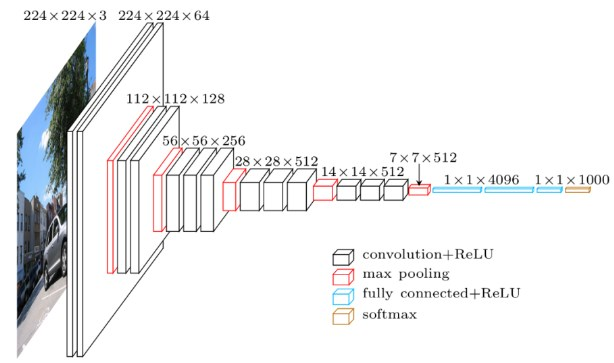
\includegraphics[scale = 0.6]{images/conv}
	\centering
	\caption{Typical outlook of a convolutional network.}
\end{figure}

The solution for this problem is the convolutional operation, of which we can take the advantage. There is a so-called sliding window that is applied on images with dot-product giving back an activation map. This map can be interpreted as something that gets activated at certain visual features. Since more convolutional layers are used, the deeper we go, the more elusive the representation of activation maps is going to be[5]. It is quite practical to use ReLU(Rectified Linear Unit)
as an activation function [6]. It actually helps prevent from having vanishing gradients through the network, at the same time being a non-linear function it imbibes complexity of the network. Its improved variant is the LeakyReLU which completely eliminates vanishing gradients problem because its derivative on the non-active side is as tiny as 0.01 or less.

\begin{figure}[!h]
	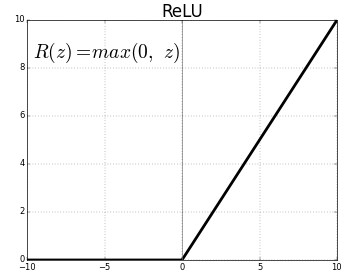
\includegraphics[scale = 0.55]{images/relu}
	\centering
	\caption{ReLU activation function}
\end{figure}

As a result of constant research many articles tried to come up with a new activation function that
can outperform ReLU function. SWISH has been released not so long ago[7]. Swish is a smooth, non-monotonic function yielding a 1 percent improvement on average compared to ReLU. Showing a proof why SWISH tackles ReLU is challenging because training is consisted of dozens of other parameteres also affecting the result of training. Regarding boundaries of SWISH, it is unbounded above, bounded below, which may lead to a significant improvement to learn underlying details of the problem.
.

\begin{figure}[!h]
	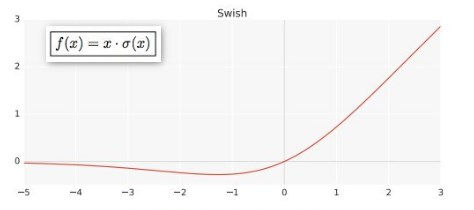
\includegraphics[scale = 0.65]{images/swish}
	\centering
	\caption{SWISH activation function}
\end{figure}

After an activation function batch normalization takes place which lets the network stabilize according to the rule of normalization, substracting the batch mean and dividing by the standard deviation. Last but not least pooling operation follows the batch normalization. Pooling layer is an important component of a CNN, because it reduces complexity of the network by downsampling. There are a few kinds which are popular, such as average, sum and max pooling operation. It assumes neighbouring pixels to have similar local properties, therefore dropping or summing some of the pixels does not have any negative effect.


\subsection{Loss function}
Role of a loss function is to measure how well our network is doing in terms of performance. If the network is poor, this function gives a high result, compared to the model that gives satisfying result because in this case smaller value is expected.
\subsubsection{Generalized dice loss function}
One of the used loss functions here is the so called Generalized Dice Score loss function, which is dedicated to applications where we come across 
highly unbalanced segmention problems [8]. It is able to supply metrics regarding how much ground truth and predicted object overlap cover one another.

\begin{equation}
\label{gdl}
GDL = 1-2\frac{\sum_{l=1}^{2}w_l\sum_{n}r_{ln}p_{ln}}{\sum_{l=1}^{2}w_l\sum_{n}r_{ln}+p_{ln}}
\end{equation} 

The loss function is defined by the equeation above, where $r_l$ is reference foreground segmentation, and $p_l$ is theprobabilistic map for the foreground, $w_l$ is to provide invariance to different label set properties.


\subsubsection{Charbonnier loss function}
Another loss function what we have applied during the training is the Charbonnier \ref{char}, or Pseudo-Huber loss since it resembles to the original Huber function featuring quadratic properties close to the minimum and linear as going further from it. Charbonnier loss is a compound of L2 and L1 loss functions, in the vicinity of minimum it tends to be convex, but far from the equilibrium it is not that steep [9]. Steepness can be affected by fine-tuning delta value. Its derivative is continious all the way.
It can be written in the following form:

\begin{equation}
\label{char}
L_\delta(a) = \delta^{2}(\sqrt{1+{(\frac{a}{\delta})^2}}-1)
\end{equation} 



\subsection{Convolutional U-NET}

Concept of U-NET convolutional network was applied in our application which had initially been developed for biological segmentation purposes at University of Freiburg [10]. Since it is meant to determine which pixel belongs to which class, it is also called fully connected convolutional network, despite of not containing any fully connected network. Having such an extension, it can work with less training examples even though performance does not get worse. The network consists of an encoder and a decoder part. Layers which represent high  resulution are in conjunction with upsampled part for localization purposes. [10]

\begin{figure}
	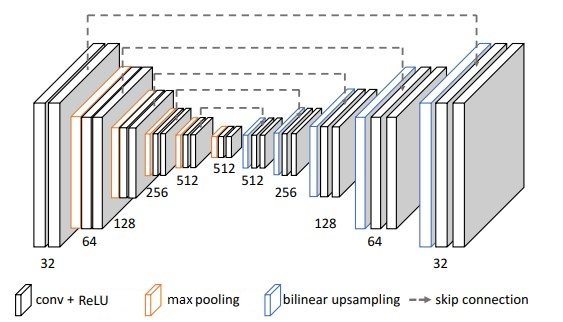
\includegraphics[scale = 0.7]{images/unet}
	\centering
	\caption{Built-up of convolutional U-NET}
\end{figure}

\subsection{ADAM optimizer}
Adam (Adaptive moment estimation) is a manifestation of stochastic gradient-based optimization which requires only the first derivative of the error function. Its power comes from two adaptive learning rates being calculated from first and second momentum of the gradients. It combines AdaGrad, which works well with sparse gradients, and RMSProp, which works well in on-line and non-stationary settings [11].


\section{Realization of the task}
\subsection{Dataset}

During our work DAVIS dataset has been used for training, testing and validating. DAVIS stands for Densely Annotated VIdeo Segmentation, containing relatively high quality videos (480p). One of the benefits of using this dataset is that, for each frame a pixel-accurate and densely annoted ground truth are provided. Generalization was also a key part in this project, and this dataset has many recordings related to common activities like walking, hockey, tennis etc.

\subsection{Data structure}
In order to make the network learn efficiently, data preprocessing is indispensable just like in every deep neural network related task. We used the image sequences of each videos in the DAVIS dataset. Having so many frames, we decided to build up an hdf5 container enabling us to handle data more conviniently The dateset was split up in a way of 70\% training, 20\% validation and 10\% test data. The concept was to take three iamges of a sequence at once, the first and last go into an input array, while the middle is considered as the output. This process goes along until we run out of pictures. The list of samples is shuffled so as to avoid any correlation between the elements. Even though the samples are kept as binaries, they are still too large to load all of them into memory, therefore implementing a fitgenerator was also a necessity. If doing so, we cannot just simply save space, but during training the fitgenerator can make up images (data augmention), feeding the DNN with new data in order to learn more efficiently.

\subsection{Training}
Based on the statements defined above, using the mentioned loss-functions and network structures we trained the network using those in different combinations. As described previously ADAM was used as general training optimizer. At a traning phase many parameters have to be adjusted. We used a constant 16 batch size for each training. The ADAM optimiter's learning rate was 0.001, with $\beta_1 = 0.9$, $\beta_2=0.999$ and $\epsilon=10^{-8}$. We tried both ReLu and Swish activation functions. We ran the training for 100 epochs. If validation loss did not improve for 6 epochs, then the learning rate was reduced to its half.



\subsection{Evaluation on a video sequence and testing}

Reaching the testing phase, having U-NET trained, a randomly video has been taken to evaluate the quality of the network. Since the videos in the DAVIS dataset are general enough, the input videos do not have to have a 15 frame rate in order to work correctly. It can also be used to upscale a 60 fps video to a 120 fps one, thus making slow motion videos are achivable as well. Some results can be seen in figure 5 and 6.

It's clearly visible that the worse performance belongs to the networks that contained SWISH activation function. Using Charbonnier loss function produced a better prediction. It can be seen in the pictures that using SoftDice the edges are not sharp enough. Our implementation with Charbonnier and ReLu seems to have produced a better quality frame prediction than the DeepMotion's, thus the generated videos are smoother as well.

\begin{figure}%
	\centering
	\subfloat[Ground Truth]{{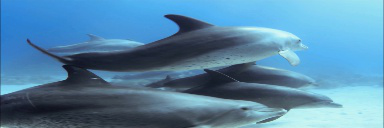
\includegraphics[width=5cm]{images/dolph_orig} }}%
	\qquad
	\subfloat[DeepMotion prediction]{{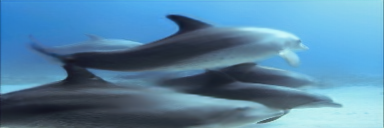
\includegraphics[width=5cm]{images/deepmotion_dolph_pred} }}%
	\qquad
	\subfloat[Charbonnier,ReLu]{{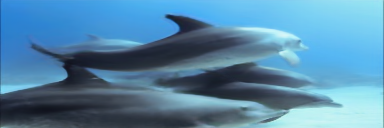
\includegraphics[width=5cm]{images/our_dolph_pred_cb_relu} }}%
	\qquad
	\subfloat[Charbonnier, SWISH]{{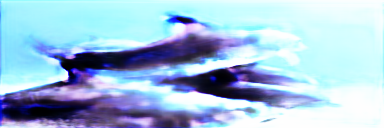
\includegraphics[width=5cm]{images/our_dolph_pred_cb_swish} }}%
	\qquad
	\subfloat[SoftDice,ReLu]{{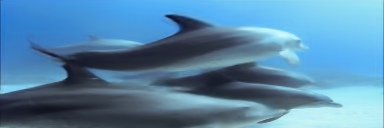
\includegraphics[width=5cm]{images/our_dolph_pred_sd_relu} }}%
	\qquad
	\subfloat[SoftDice,SWISH]{{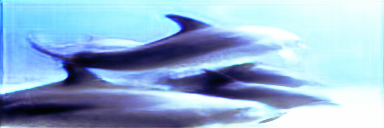
\includegraphics[width=5cm]{images/our_dolph_pred_sd_swish} }}%
	\caption{Prediction for dolphines}%
	\label{fig:example}%
\end{figure}

\begin{figure}%
	\centering
	\subfloat[Ground Truth]{{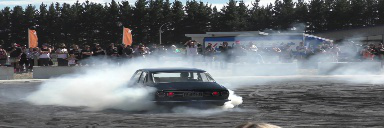
\includegraphics[width=5cm]{images/drift_orig} }}%
	\qquad
	\subfloat[DeepMotion prediction]{{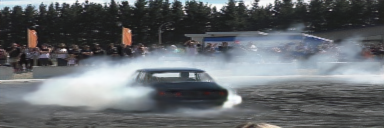
\includegraphics[width=5cm]{images/deepmotion_drift_pred} }}%
	\qquad
	\subfloat[Charbonnier,ReLu]{{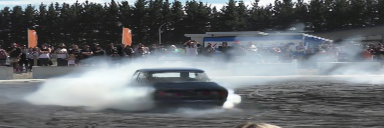
\includegraphics[width=5cm]{images/our_drift_pred_cb_relu} }}%
	\qquad
	\subfloat[Charbonnier, SWISH]{{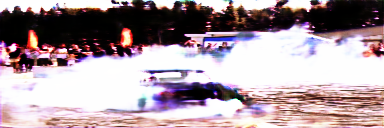
\includegraphics[width=5cm]{images/our_drift_pred_cb_swish} }}%
	\qquad
	\subfloat[SoftDice,ReLu]{{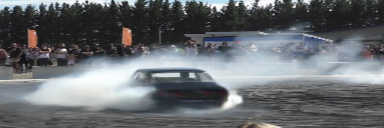
\includegraphics[width=5cm]{images/our_drift_pred_sd_relu} }}%
	\qquad
	\subfloat[SoftDice,SWISH]{{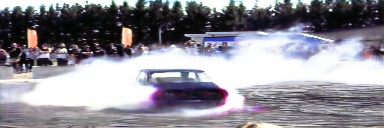
\includegraphics[width=5cm]{images/our_drift_pred_sd_swish} }}%
	\caption{Prediction for drifting car}%
	\label{fig:example}%
\end{figure}

The loss and accuracy curves for each network can be seen in figures 7 and 8. It can be seen, that using SWISH the network produces a higher accuracy and better loss value, however this is not what we can see on the pictures.
\begin{figure}[H]%
	\centering
	\subfloat[Charbonnier, ReLu]{{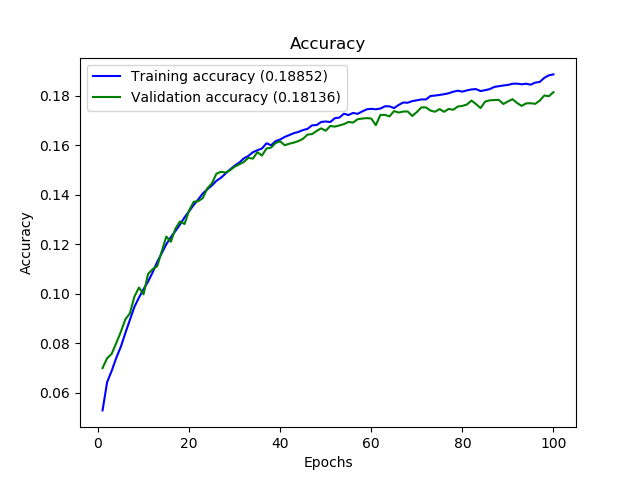
\includegraphics[width=6cm]{images/cb_relu_acc} }}%
	\qquad
	\subfloat[Charbonnier, SWISH]{{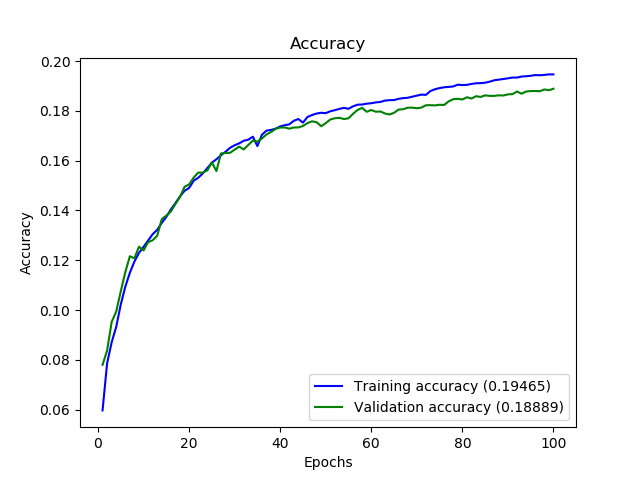
\includegraphics[width=6cm]{images/cb_swish_acc} }}%
	\qquad
	\subfloat[SoftDice, ReLu]{{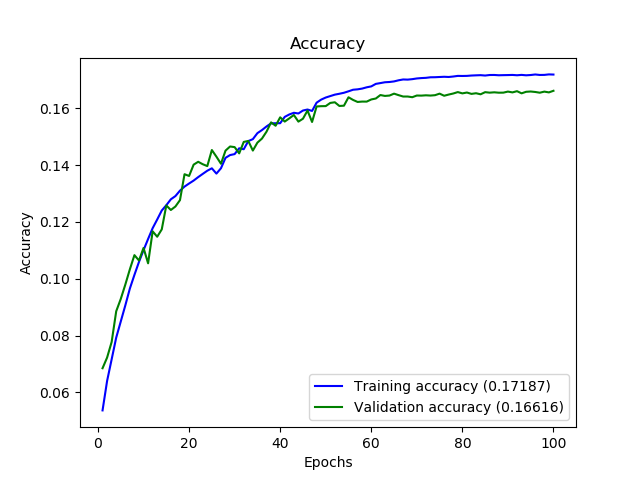
\includegraphics[width=6cm]{images/sd_relu_acc} }}%
	\qquad
	\subfloat[SoftDice, SWISH]{{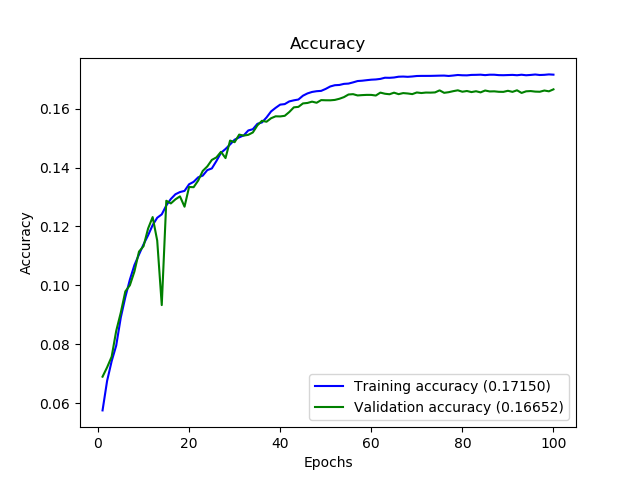
\includegraphics[width=6cm]{images/sd_swish_acc} }}%
	\caption{Accuracy curves}%
	\label{fig:example}%
\end{figure}

\begin{figure}[H]%
	\centering
	\subfloat[Charbonnier, ReLu]{{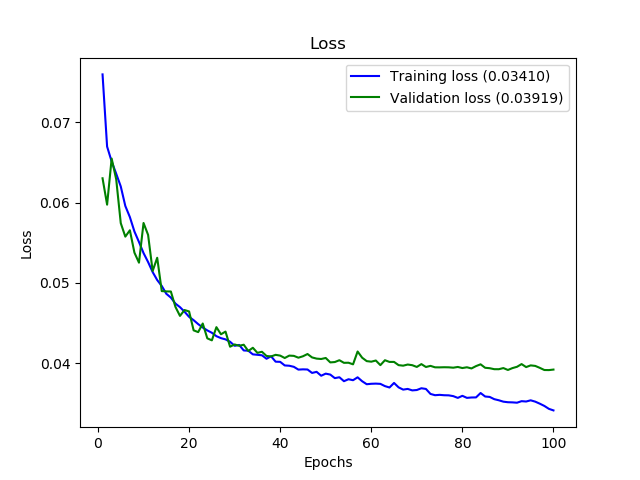
\includegraphics[width=6cm]{images/cb_relu_loss} }}%
	\qquad
	\subfloat[Charbonnier, SWISH]{{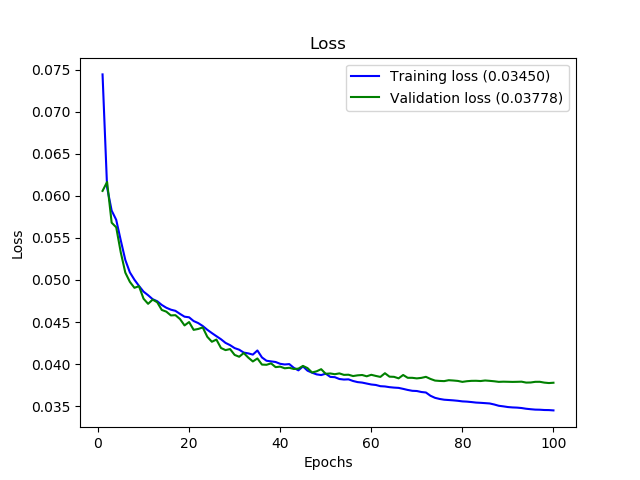
\includegraphics[width=6cm]{images/cb_swish_loss} }}%
	\qquad
	\subfloat[SoftDice, ReLu]{{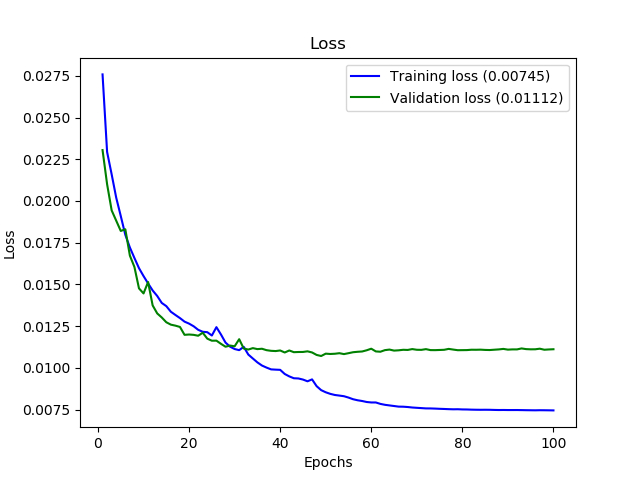
\includegraphics[width=6cm]{images/sd_relu_loss} }}%
	\qquad
	\subfloat[SoftDice, SWISH]{{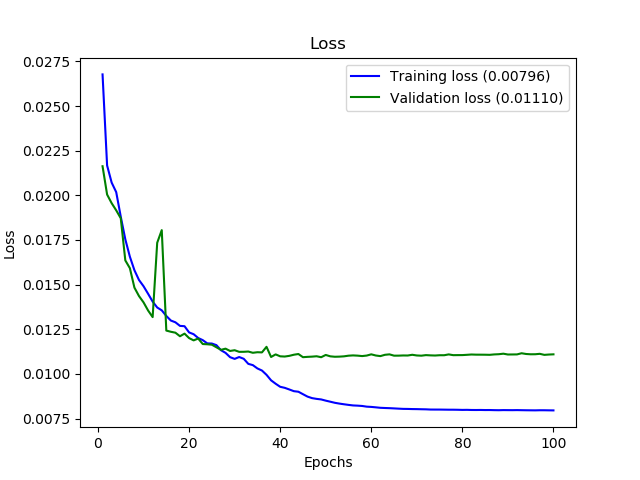
\includegraphics[width=6cm]{images/sd_swish_loss} }}%
	\caption{Loss curves}%
	\label{fig:example}%
\end{figure}

\section{Conclusion, further improvements}
From the pictures above we can see that our method works better than the arcticle on which our idea is based on. The improvement is due to the usage of more sophisticated loss function. It's clear that the predictions have the worst performance around sharp edges and lines on the pictures. Using SWISH activation function does not seem to be efficient for frame rate upscaling. We got the worst performanceusing Charbonnier loss function with SWISH activation. The difference between networks trained with Charbonnier and SoftDice loss function can not be cleary seen in the images, however, we could see the effects of smooth edges in a video. In the future, developing a loss function which gives greater "penalty" for differences around these features would be reasonable. Further investigation of several activation functions might also lead to a great improvement.

\section*{References}
\medskip

\small

[1] K. Hilman, H. Park, Y. Kim, IEEE Trans. Circuits Syst. Video Technol.
10 (6) (2000) 869e877.

[2] Chuanxin Tang, Ronggang Wang, Zhu Li b, Wenmin Wang, Wen Gao (2016). Frame interpolation with pixel-level motion vector field and mesh based
hole filling

[3]E. Ilg, N. Mayer, T. Saikia, M. Keuper, A. Dosovitskiy, and
T. Brox. Flownet 2.0: Evolution of optical flow estimation
with deep networks. In CVPR, 2017

[4] Huaizu Jiang, Deqing Sun, Varun Jampani, Ming-Hsuan Yang, Erik Learned-Miller, Jan Kautz(2018).: 
Super SloMo: High Quality Estimation of Multiple Intermediate Frames
for Video Interpolation

[5] Krizhevsky, A., Sutskever, I., \& Hinton, G. E. (2012).
Imagenet classification with deep convolutional neural
networks. In Advances in neural information processing
systems (pp. 1097-1105).

[6] Xavier Glorot, \& Antoine Bordes \& Yoshua Bengio (2011).Deep Sparse Rectifier Neural Networks

[7] Prajit Ramachandran \& Barret Zoph \& Quoc V. Le(2017).
SWISH: A SELF-GATED ACTIVATION FUNCTION

[8]Carole H. Sudre, Wenqi Li, Tom Vercauteren, Sebastien Ourselin, M. Jorge Cardoso (2017.)
Generalised Dice overlap as a deep learning loss
function for highly unbalanced segmentations

[9] Jonathan T. Barron(2018).
A General and Adaptive Robust Loss Function

[10] Olaf Roneberger, Philipp Fischer, Thomas Brox(2015).
U-Net: Convolutional Networks for Biomedical Image Segmentation

[11] Kingma, D., \& Ba, J. (2014). Adam: A method for stochastic
optimization

[12] Neil Joshi, Duncan Woodbury, \&  (2014) A convolutional Neural Network for Frame interpolation

\end{document}